\chapter{Métodos e Procedimentos}
Neste capítulo será exposto o trabalho desenvolvido quanto da elaboração dos projetos das NFPs e das medidas realizadas, será mostrado a metodologia adotada para a concepção dos leiautes das NFPs, discorrerá-se-á sobre os equipamentos de laborátorio necessários e utilizados na realização das medidas de caracterização e por fim será abordado a metodologia utilizada na caracterização das NFPs.

\section{Topologias de leiaute desenvolvidas}
A Partir do estudo realizado no capítulo~\ref{fundamentacao} conhecia-se de antemão algumas topologias de leiaoute de NFPs, sabia-se, por exemplo, que em regra geral uma NFP para campo magnético próximo, deveria possuir essencialmente duas partes, uma espira (para detecção do campo magnético) e uma linha de transmissão (para conduzir o sinal capturado). Diante deste cenário, estabeleceu-se como critério a utilização de espiras com raios diferentes, no intuito de verificar a influência do raio (tamanho da espira) na sensitividade. Outro critério foi a verificação da influência do plano de terra na sensitividade e largura de banda das NFPs e como último critério a adoção de PCIs de face dupla, afim de utilizar 2 espiras (uma em cada face) e verificar a influência do numero de espiras nas caracteristicas das NFPs.

Com isso, desenvolveu-se ao todo 12 NFPs separadas em dois grupos, leiautes de face simples e leiautes de face dupla. Para cada grupo destes, utilizou-se três tamanhos de raios, 0.5mm, 1mm e 1.5mm, e para cada raio desenvolveu-se uma NFP com e sem o plano de terra, assim o rol de NFPs desenvolvidas pode ser enumerado da seguinte forma:

\begin{enumerate}
 \item Leiautes de Face Simples:
 \begin{itemize}
  \item 1A: Face simples com raio de 0.5 mm sem o plano de terra.
  \item 1B: Face simples com raio de 0.5 mm com o plano de terra.
  \item 2A: Face simples com raio de 1 mm sem o plano de terra.
  \item 2B: Face simples com raio de 1 mm com o plano de terra.
  \item 3A: Face simples com raio de 1.5 mm sem o plano de terra.
  \item 3B: Face simples com raio de 1.5 mm com o plano de terra.
 \end{itemize}
 
  \item Leiautes de Face Dupla:
 \begin{itemize}
  \item 4A: Face dupla com raio de 0.5 mm sem o plano de terra.
  \item 4B: Face dupla com raio de 0.5 mm com o plano de terra.
  \item 5A: Face dupla com raio de 1 mm sem o plano de terra.
  \item 5B: Face dupla com raio de 1 mm com o plano de terra.
  \item 6A: Face dupla com raio de 1.5 mm sem o plano de terra.
  \item 6B: Face dupla com raio de 1.5 mm com o plano de terra.
 \end{itemize}
\end{enumerate}

Rede de Ponta de Pronta

\subsection{Projeto das NFPs}
O leiaoute das sondas foi desenvolvido utilizando o software CAD Altium\textregistered, incluiu-se no circuito uma carga resistiva de $50\Omega$ afim de casar impedância com os analisadores de espectro e geradores de funções (Equipamentos utilizados na caracterização).

Na figura~\ref{fig:1A_layers} pode-se visualizar o leiaoute desenvolvido para a NFP de face simples com raio de 0.5mm sem o plano de terra. Na figura~\ref{fig:1B_layers} pode-se visualizar o leiaoute desenvolvido para a NFP de face simples com raio de 0.5mm com o plano de terra.
\begin{figure}[htb!]
	\centering
 	\caption{NFP face simples - 0.5mm}
	\subfloat[][1A - Sem plano de terra]{
		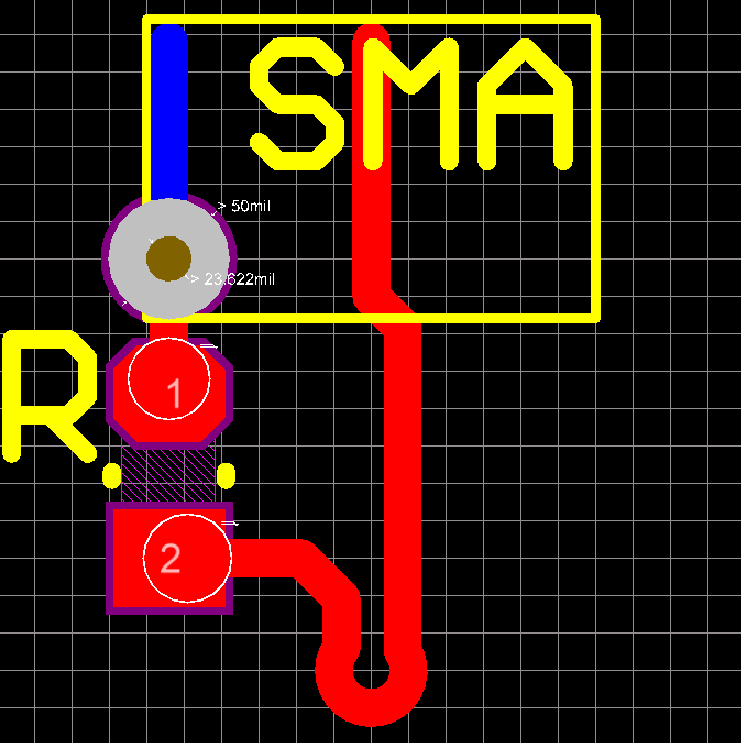
\includegraphics[scale=0.35]{./img/1A_layers}
		\label{fig:1A_layers}}
	\subfloat[][1B - Com plano de terra]{
		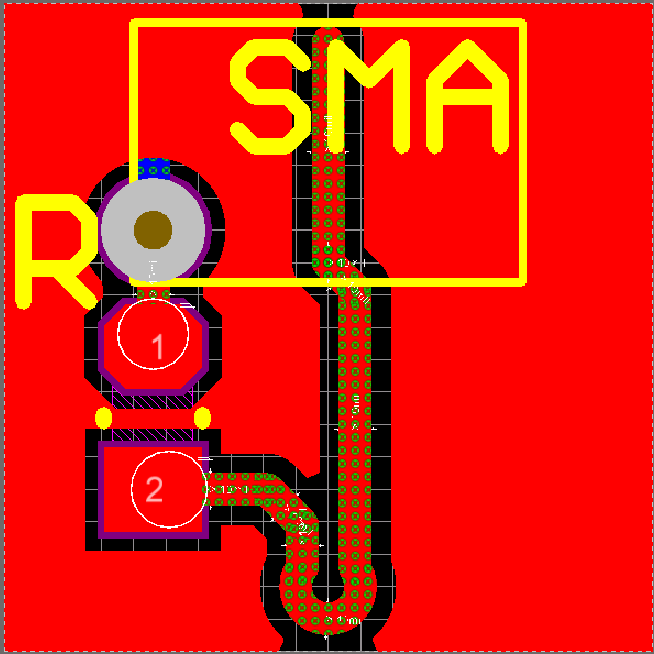
\includegraphics[scale=0.4]{./img/1B_layers}
		\label{fig:1B_layers}}
    \fonte{Elaborado pelo Autor}
\end{figure}

Na figura~\ref{fig:2A_layers} pode-se visualizar o leiaoute desenvolvido para a NFP de face simples com raio de 1mm sem o plano de terra. Na figura~\ref{fig:2B_layers} pode-se visualizar o leiaoute desenvolvido para a NFP de face simples com raio de 1mm com o plano de terra.
\begin{figure}[htb!]
	\centering
 	\caption{NFP face simples - 1mm}
	\subfloat[][2A - Sem plano de terra]{
		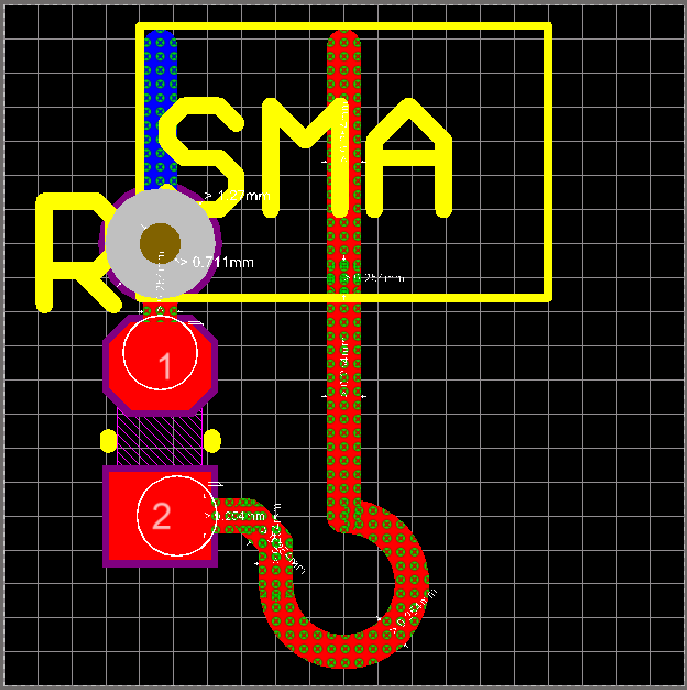
\includegraphics[scale=0.4]{./img/2A_layers}
		\label{fig:2A_layers}}
	\subfloat[][2B - Com plano de terra]{
		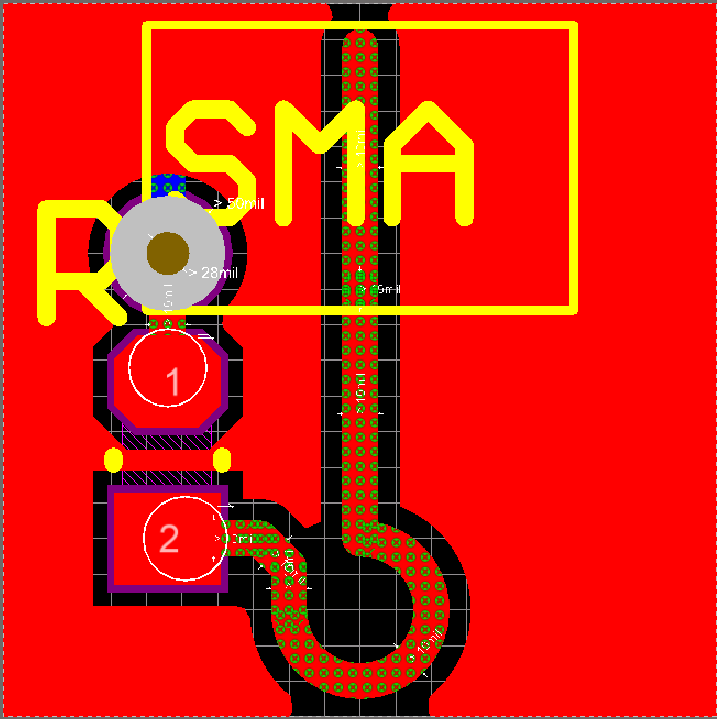
\includegraphics[scale=0.38]{./img/2B_layers}
		\label{fig:2B_layers}}
    \fonte{Elaborado pelo Autor}
\end{figure}

Na figura~\ref{fig:3A_layers} pode-se visualizar o leiaoute desenvolvido para a NFP de face simples com raio de 1.5mm sem o plano de terra. Na figura~\ref{fig:3B_layers} pode-se visualizar o leiaoute desenvolvido para a NFP de face simples com raio de 1.5mm com o plano de terra. Como o raios desta NFP ficou 3 vezes maior que as~\ref{fig:1A_layers} e~\ref{fig:1B_layers} notamos que a espira não ficou completa, faltou $\frac{1}{4}$ de volta para realizar a espira completa.
\begin{figure}[htb!]
	\centering
 	\caption{NFP face simples - 1.5mm}
	\subfloat[][3A - Sem plano de terra]{
		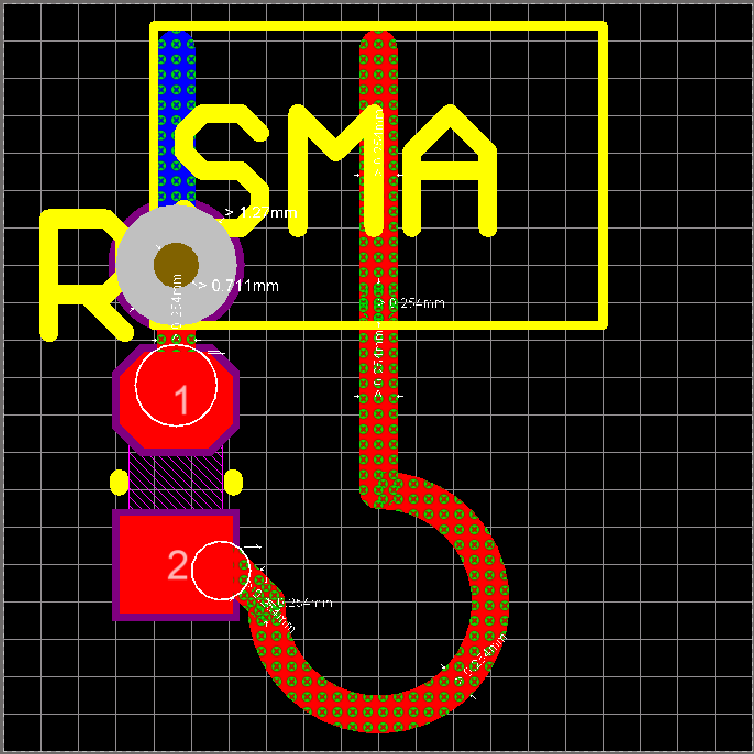
\includegraphics[scale=0.38]{./img/3A_layers}
		\label{fig:3A_layers}}
	\subfloat[][3B - Com plano de terra]{
		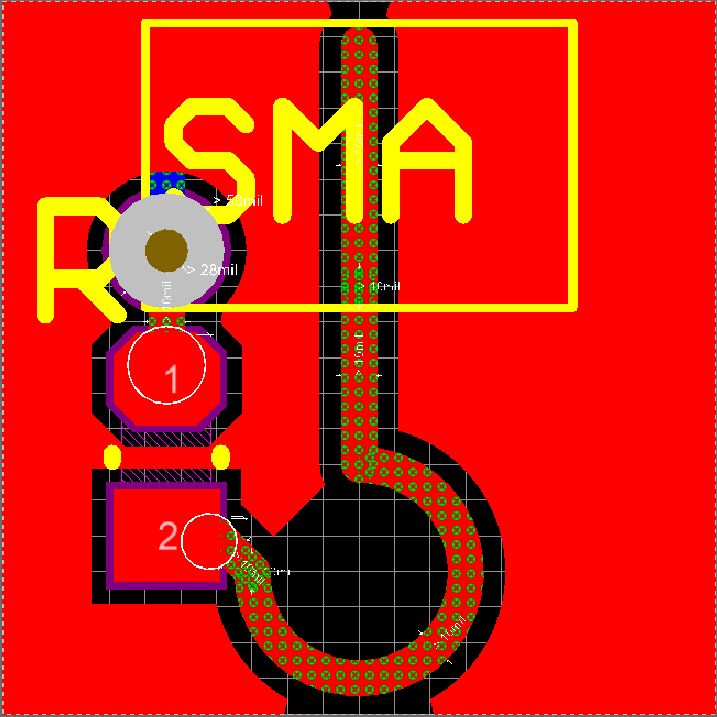
\includegraphics[scale=0.4]{./img/3B_layers}
		\label{fig:3B_layers}}
    \fonte{Elaborado pelo Autor}
\end{figure}

Desenvolvidas as NFPs de face simples, partiu-se para os leiaoutes das faces duplas. Na figura~\ref{fig:4A_layers} pode-se visualizar o leiaoute desenvolvido para a NFP de face dupla com raio de 0.5mm sem o plano de terra. Na figura~\ref{fig:4B_layers} pode-se visualizar o leiaoute desenvolvido para a NFP de face dupla com raio de 0.5mm com o plano de terra. Devido ao fato de necessitar-se de uma via (ligação entre faces) a espira desta NFP assumiu um formato eliptico, preservando-se o menor raio em 0.5mm, no sentido horizontal, porém com uma raio vertical de 2.5mm.
\begin{figure}[htb!]
	\centering
 	\caption{NFP face dupla - 0.5mm}
	\subfloat[][4A - Sem plano de terra]{
		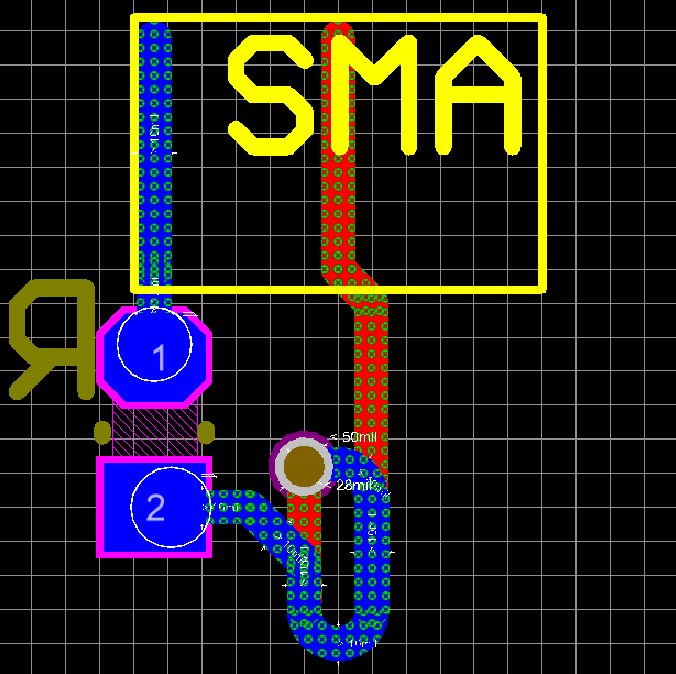
\includegraphics[scale=0.4]{./img/4A_layers}
		\label{fig:4A_layers}}
	\subfloat[][4B - Com plano de terra]{
		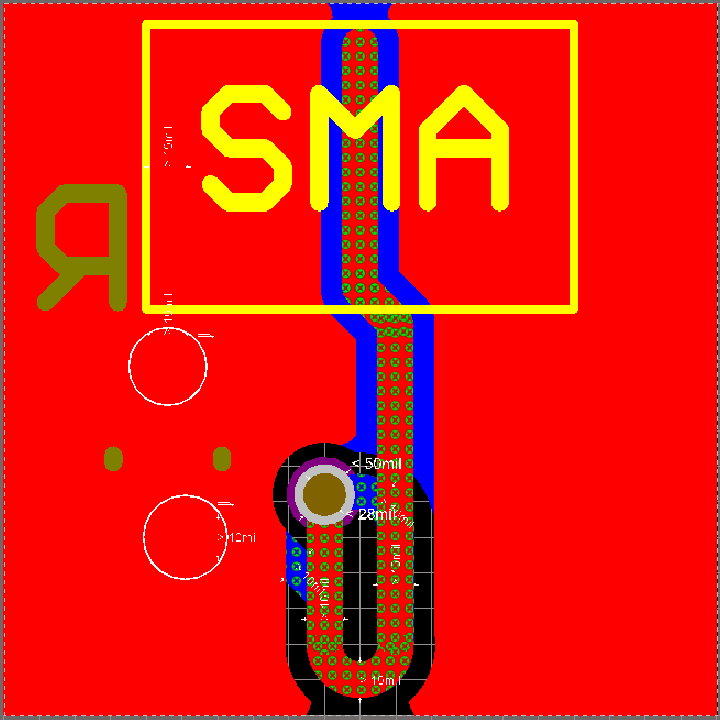
\includegraphics[scale=0.38]{./img/4B_layers}
		\label{fig:4B_layers}}
    \fonte{Elaborado pelo Autor}
\end{figure}

Na figura~\ref{fig:5A_layers} pode-se visualizar o leiaoute desenvolvido para a NFP de face dupla com raio de 1mm sem o plano de terra. Na figura~\ref{fig:5B_layers} pode-se visualizar o leiaoute desenvolvido para a NFP de face dupla com raio de 1mm com o plano de terra. 
\begin{figure}[htb!]
	\centering
 	\caption{NFP face dupla - 1mm}
	\subfloat[][5A - Sem plano de terra]{
		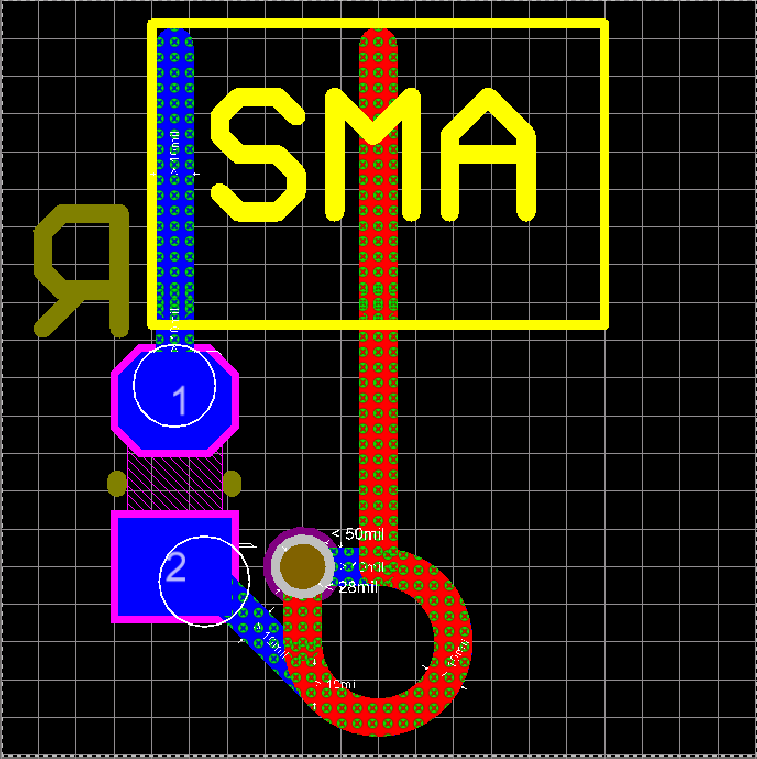
\includegraphics[scale=0.38]{./img/5A_layers}
		\label{fig:5A_layers}}
	\subfloat[][5B - Com plano de terra]{
		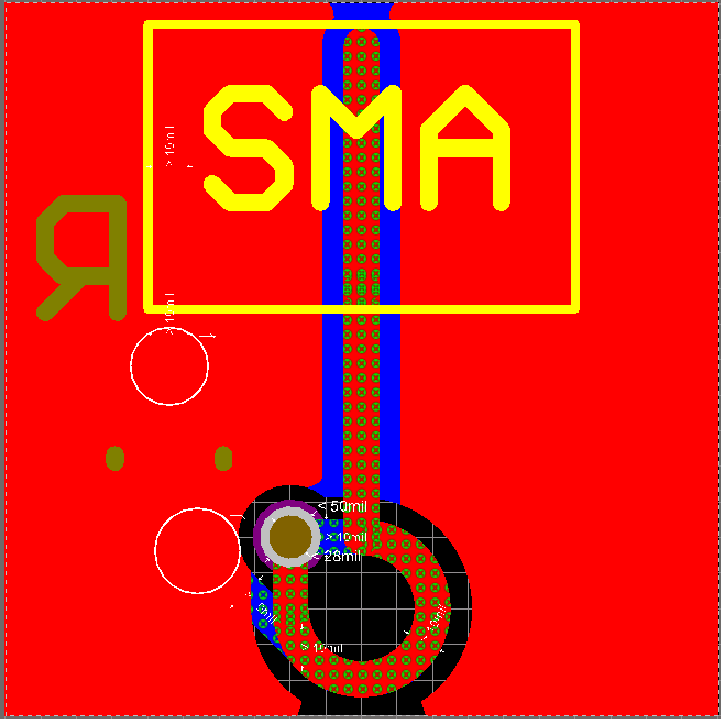
\includegraphics[scale=0.4]{./img/5B_layers}
		\label{fig:5B_layers}}
    \fonte{Elaborado pelo Autor}
\end{figure}

Na figura~\ref{fig:6A_layers} pode-se visualizar o leiaoute desenvolvido para a NFP de face dupla com raio de 1.5mm sem o plano de terra. Na figura~\ref{fig:6B_layers} pode-se visualizar o leiaoute desenvolvido para a NFP de face dupla com raio de 1.5mm com o plano de terra. Diferentemente do grupo de face simples, nota-se aqui que as NFPs de face duplas, em pelo menos 1 (uma) espira tem-se a volta completa. 
\begin{figure}[htb!]
	\centering
 	\caption{NFP face dupla - 1.5mm}
	\subfloat[][6A - Sem plano de terra]{
		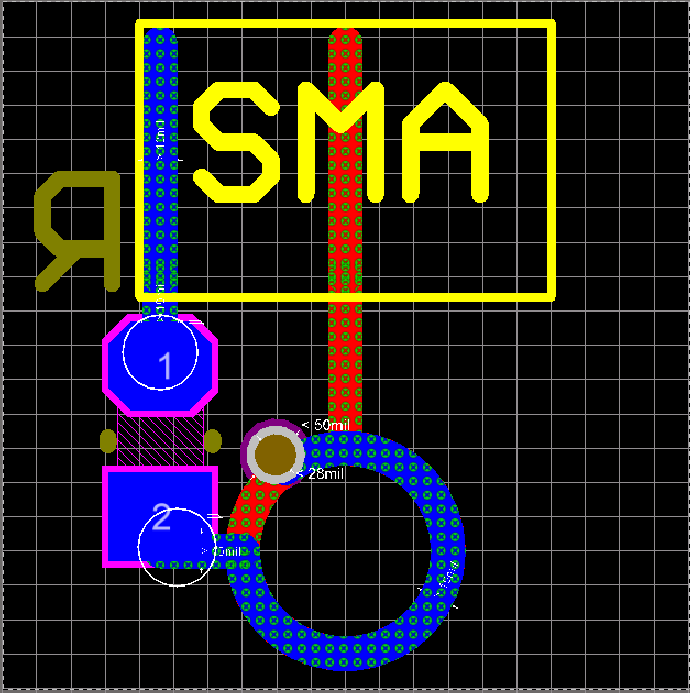
\includegraphics[scale=0.4]{./img/6A_layers}
		\label{fig:6A_layers}}
	\subfloat[][6B - Com plano de terra]{
		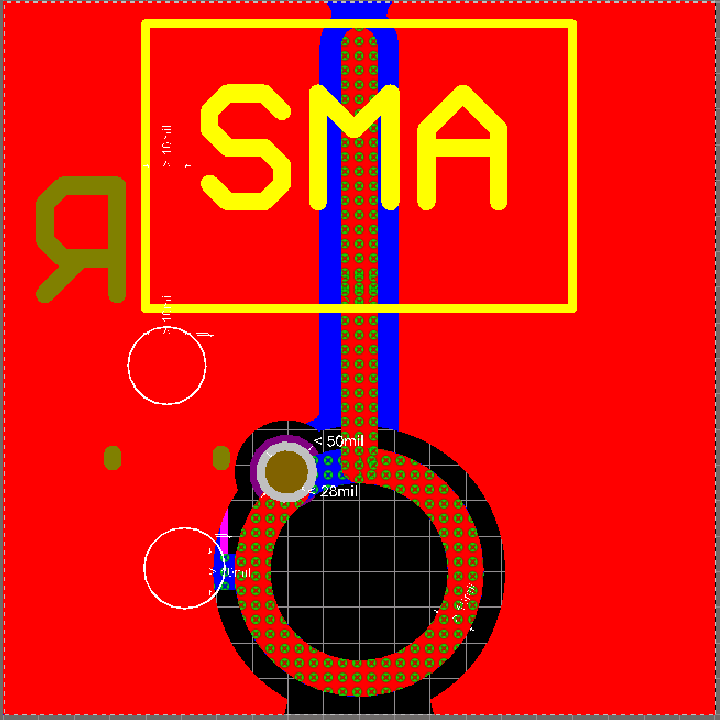
\includegraphics[scale=0.39]{./img/6B_layers}
		\label{fig:6B_layers}}
    \fonte{Elaborado pelo Autor}
\end{figure}

As maiores dificuldades nos projetos das NFPs, de forma geral, foi a alocação da carga resistiva de $50\Omega$ (Casamento de impedância) e alocar a via (ligação interfaces), esses pequenos empecilhos acarretaram na imperfeição do formato circular, fechado, das espiras, para as NFPs de raios menores que 1.5mm.

\section{Setup de medidas e procedimentos}

Fazer Desenho do SETUP de MEDIDAS (Analisador + DUT + Suporte + NFP)


Para a realização dos experimentos seria necessário, idealmente, ter um sistema de posicionamento XY, porém este sistema de posicionamento foi tratado em outro estudo desenvolvido no LabCEM, assim para realizas as experimentações, desenvolveu-se um suporte fixo em madeira (para não interferir nas radiações eletromagnéticas) em que o posicionamento da NFP se dá de forma manual.

Foto do suporte usado para as NFPs e os DUTS

Abaixo do suporte, em plano fixo, foi alocado o dispositivo sob teste (DUT).

\subsection{Modelo para o dispositivo sob teste - DUT}


\subsection{Equipamentos do laborátorio}
Falar sobre o equipamentos do Laborátorio

\begin{figure}[htb!]
	\centering 
	\caption{Analisador de Espectro - ESL}
	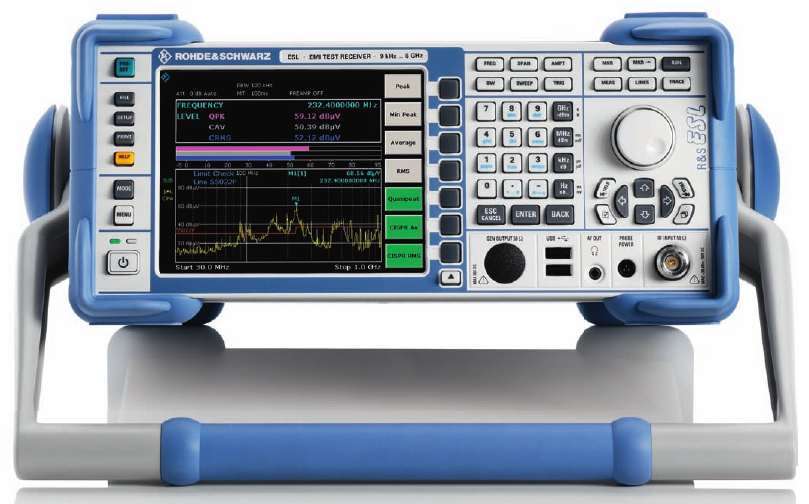
\includegraphics[scale=0.6]{./img/esl}
	\fonte{ARRUMAR Adaptado de~\citeonline{funato2006}}
	%\legend{\hspace{-218pt}Fonte:~\citeonline[p.~8]{paul2006}}
	\label{fig:esl}
\end{figure}

\section{Caracterização da resposta em frequência}

\section{Caracterização dos paramentros essencias}


\subsection{Fator de Antena}

\subsubsection*{Leiaoutes de face simples}

\subsubsection*{Leiaoutes de face supla}


\subsection{Sensitividade}

\subsubsection*{Leiaoutes de face simples}

\subsubsection*{Leiaoutes de face supla}


\subsection{Seletividade}

\subsubsection*{Leiaoutes de face simples}

\subsubsection*{Leiaoutes de face supla}


\subsection{Resolução Especial}

\subsubsection*{Leiaoutes de face simples}

\subsubsection*{Leiaoutes de face supla}


\subsection{Largura de Banda}

\subsubsection*{Leiaoutes de face simples}

\subsubsection*{Leiaoutes de face supla}

